\section{一些技巧}

这里所指技巧具有专题性的意义,是面向解决方案的,而不是面向功能的讲解。





\subsection{内存溢出及解决方案}

\paragraph{内存溢出}所谓内存溢出,也就是计算时出现的 Out of memoery.

\begin{figure}[htbp]
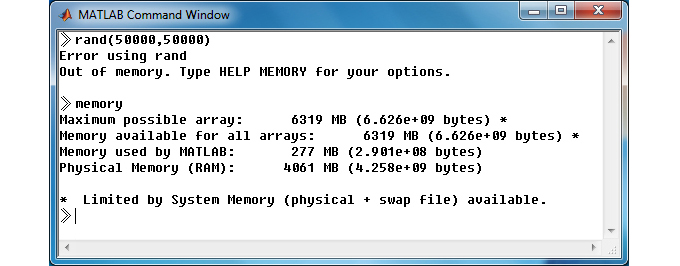
\includegraphics[width=0.6\textwidth]{memoryout}
\caption{内存溢出和内存查看}
\end{figure}

\vspace{-0.8cm}
\lstinputlisting[language=matlab, caption={生成随机矩阵测试内存溢出}]{secSkillsSome/rand-matrix.m}

\notation{逐渐增大或减小维数,这样可以测试设备能存储最大矩阵的维数。}


\paragraph{内存溢出解决} 简而言之,开源节流。

\begindot
  \item 开源方法
    \begin{itemize*}
    \item 增加RAM。买个大点的内存条装上;
    \item 以“no java”方式启动MATLAB。(这是在节MATLAB的流,开程序执行的源)
    \end{itemize*}
  \item 节流方法
    \begin{itemize*}
    \item 数据本地存储。将数据存储到本地,需要时再导入;
    \item 使用已有的变量,即时删除临时变量(不再需要的变量);
    \item 以函数封装。将程序中某几部分的代码封装为 function 调用,function 调用只输出最后需要的数据,其间的临时变量在每次调用完 function 之后都会自动删除。
    \end{itemize*}
\myenddot





\subsection{自定义函数帮助}

在MATLAB中可以用输入help加函数名来获得获悉使用方法及例子。我们期望对自己编写的函数也实现这样的功能,那么有两个关键点,一是参照MATLAB的内置函数注释格式写好注释(或者参照下面的示例),二是确保此函数路径已经添加。接下来就可以通过 \mcode{help myfunction} 这样的形式来查看了。

\vspace{-0.8cm}
\lstinputlisting[language=matlab, caption={自定义帮助}]{secSkillsSome/define-help-comment.m}





\subsection{图像导出}

除了一般的截图方法,有这样几种方法。

\begindot
  \item \mcode{print('-dpdf',pdf_name);},生成图像为pdf格式。
  \item 直接设置导出, File - Export Setup - Export,通过 Rendering - Resolution 可以设置图像质量。
  \item \mcode{saveas(gcf, 'output', 'jpg')},导出当前figure为名为output的jpg格式图像。
\myenddot





\subsection{公式打印}
MATLAB 支持 \LaTeX 的公式输出,在两个地方可能用到公式输出。

\begindot
  \item 图片上的公式。
  \item 代码发布注释中的公式。
\myenddot

\vspace{-0.8cm}
\lstinputlisting[language=matlab, caption={图像中的公式输出}]{secSkillsSome/math-in-figure.m}





\subsection{重复向量以构造矩阵}

首先解释一下什么是向量重复构造矩阵(并非是一个专业术语),比如有一个向量 \mcode{[1 2 3]},现在我打算将它构造成 \mcode{[1 2 3; 1 2 3; 1 2 3]},这就是此小节要解决的内容。

\vspace{-0.8cm}
\lstinputlisting[language=matlab, caption={重复向量以构造矩阵}]{secSkillsSome/repeat-matrix.m}

\vspace{-0.8cm}
\lstinputlisting[language=matlab, nolol]{secSkillsSome/repeat-matrix-result.m}


实际上,\mcode{repmat} 用到了第三种,在其源码中可以看的到,但它更加通用。如果是数值,首推第三者。
 \mcode{repmat} 的源码可以通过 \mcode{which repmat} 查看其位置。另外需要提及,测试时每段前面当加 \mcode{clear},这是要消除由于内存的原因影响后面程序的执行效率。\par

还有一种方式,这种方式可以列重复挨着:

\vspace{-0.4cm}
\lstinputlisting[language=matlab, nolol]{secSkillsSome/repeat-matrix-2.m}

\notation{可以考虑用上面的某种方法用向量重复来构造三维的矩阵。}